\documentclass[fleqn]{exam}

\usepackage{fullpage}
\usepackage{enumerate}
\usepackage{unitsdef} 
\usepackage{graphicx}
\usepackage[fleqn]{mathtools}
\usepackage{cancel}
\usepackage{polynom}
\usepackage{float}
\usepackage{mdwlist}
\usepackage{booktabs}
\usepackage{cancel}
\usepackage{polynom}
\usepackage{caption}

\setlength{\mathindent}{.5 cm}

\everymath{\displaystyle}

% \begin{figure}[H]
%   \centering
%   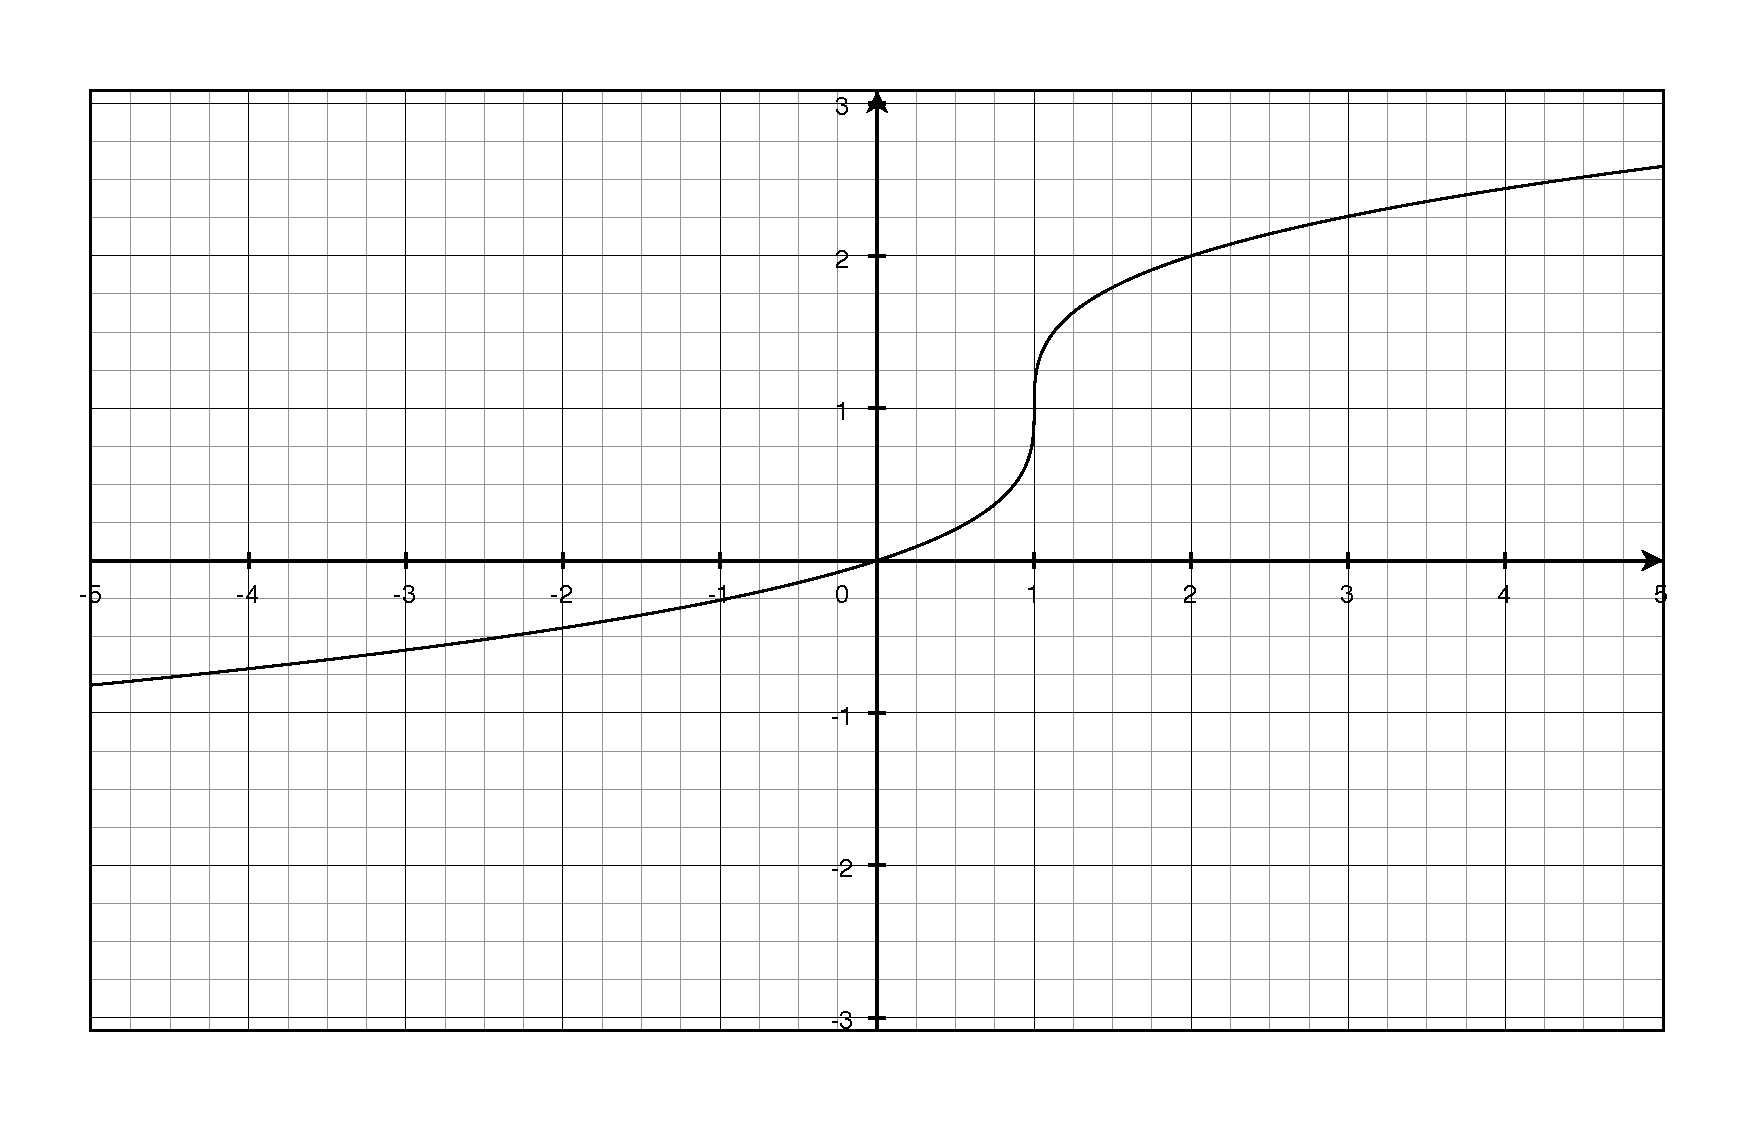
\includegraphics[scale=.3]{question7.eps}
%   \caption*{Question 7}
% \end{figure}

% \begin{tabular}{cc}
% \toprule
% period & amplitude \\
% \midrule
%   $\pi$ & $2$ \\
% \bottomrule
% \end{tabular}

\newunit{\inch}{in}
\newunit{\mile}{mile}
\newunit{\foot}{ft}
\newunit{\knot}{knot}
\newunit{\gallon}{gallon}

\printanswers

\ifprintanswers 
\usepackage{2in1, lscape} 
\fi

\title{Math 263A \\ Homework 13}
\date{May 2, 2012}

\begin{document}

\maketitle

\section{Homework}

\begin{itemize*}
  \item Read Section 4.2
  \item pp. 187-188: 1-5, 7, 10-15, 17, 19-20, 22-23, 25, 31, 33
\end{itemize*}

\section{Review}
\begin{questions}


\question
Evaluate the limit:
\[
  \lim_{x \to 1} \left( \frac{x^2}{x-1} - \frac{1}{x-1} \right)
\]

\begin{solution}
\begin{align*}
  \lim_{x \to 1} \left( \frac{x^2}{x-1} - \frac{1}{x-1} \right) &= \lim_{x \to 1} \frac{x^2 - 1}{x-1} \\
  &= \lim_{x \to 1} \frac{\cancel{(x - 1)}(x+1)}{\cancel{(x-1)}} \\
  &= \lim_{x \to 1} x+1 \\
  &= 2 \\
\end{align*}
\end{solution}

\question
Evaluate the limit:
\[
  \lim_{x \to 2} \frac{1/x - 1/2}{x - 2}
\]

\begin{solution}
\begin{align*}
  \lim_{x \to 2} \frac{1/x - 1/2}{x - 2} &=  \lim_{x \to 2} \frac{ \left( \cfrac{2 - x}{2x} \right) }{x - 2} \\
   &=  \lim_{x \to 2} \frac{2 - x}{2x(x - 2)} \\
   &=  \lim_{x \to 2} \frac{- \cancel{(x - 2)}}{2x \cancel{(x - 2)}} \\
   &=  \lim_{x \to 2} \frac{-1}{2x} \\
   &=  - \frac{1}{4} \\
\end{align*}
\end{solution}

\question
Find the point $P$ on the graph $y = x^3$ such that the tangent line at $P$ has an x-intercept of 4.

\begin{solution}
Call the point we're looking for: $P = (x_0, y_0)$

Start with the tangent line.  The x-intercept of 4 tells us that the equation for the line is:
\[
  y = m(x-4)
\]

We know that the slope is the derivative of the original equation:
\[
  m = 3x^2
\]

We can put all this information together to find $x_0$:
\begin{align*}
  x_0^3 &= 3x_0^2(x_0 - 4) \\
  x_0^3 &= 3x_0^3 - 12x_0^2 \\
  x_0 &= 3x_0 - 12 \\
  x_0 &= 6 \\
\end{align*}

So the point is: $P = (6, 216)$

\end{solution}

\end{questions}

\section{Extra Credit}
page 188, problem 38

\begin{solution}

If 
\[
f(x) = ax^3 + bx^2 + cx + d
\]
then 
\[
  f'(x) = 3ax^2 + 2bx + c
\]

$f'$ is a parabola.  The only way for a parabola to be always on or above the x-axis is if:
\begin{itemize*}
  \item the coefficient of the $x^2$ term is positive so the parabola opens upward.
  \item it never crosses below the x axis, which means it has 0 or one solutions.
\end{itemize*}

We can find the solutions to $f'(x) = 0$ using the quadratic formula:
\[
  x = \frac{-2b \pm \sqrt{4b^2 - 12ac}}{6a}
\]

For there to be no solution or only one solution, the value inside the square root must be 0 or negative:
\begin{align*}
  4b^2 - 12ac &\leq 0 \\
  |b| &\leq \sqrt{3ac} \\
\end{align*}

So the conditions for $f$ do be always increasing are: $a > 0$ and $- \sqrt{3ac} \leq b \leq \sqrt{3ac}$

\end{solution}

\ifprintanswers

\section{Homework}

\begin{description}

\item[1]
\begin{align*}
  f(x)  &= 3x + 3 \\
  f'(x) & = 3 \\
\end{align*}

$f'$ is always positive so the $f$ is always increasing.

\item[2]
\begin{align*}
  g(x)  &= (x + 1)(x - 2) \\
        &= x^2 - x - 2 \\
\\
  g'(x) & = 2x - 1 \\
  2x - 1 &\geq 0 \\
  2x &\geq 1 \\
  x &\geq \frac{1}{2}
\end{align*}

\begin{tabular}{ll}
\toprule
increasing & decreasing \\
\midrule
$\left[\frac{1}{2}, \infty \right)$ & $\left( -\infty, \frac{1}{2} \right]$ \\
\bottomrule
\end{tabular}

\item[3]
\begin{align*}
  h(t) &= t^2 + 2t - 2 \\
\\
  h'(t) & = 2t + 2 \\
  2t + 2 &\geq 0 \\
  t &\geq -1 \\
\end{align*}

\begin{tabular}{ll}
\toprule
increasing & decreasing  \\
\midrule
$[-1, \infty)$ & $( -\infty, -1]$  \\
\bottomrule
\end{tabular}

\item[4]
\begin{align*}
  f(x) &= x^3 - 1 \\
\\
  f'(x) & = 3x^2 \\
  3x^2 &\geq 0 \\
  x^2 &\geq 0 \\
\end{align*}

$f$ is always increasing.

\item[5]
\begin{align*}
  G(x) &= 2x^3 - 9x^2 + 12x \\
\\
  G'(x) & = 6x^2 - 18x + 12 \\
  6x^2 - 18x + 12 &\geq 0 \\
  x^2 - 3x + 2 &\geq 0 \\
  (x - 2)(x - 1) &\geq 0 \\
\end{align*}

\begin{tabular}{ll}
\toprule
increasing & decreasing \\
\midrule
$( -\infty, 1] \cup [2, \infty]$ & $[1, 2]$ \\
\bottomrule
\end{tabular}

\item[7]
\begin{align*}
  h(z) &= \frac{z^4}{4} - \frac{4z^3}{6} \\
\\
  h'(z) & = z^3 - 2z^2 \\
  z^3 - 2z^2 &\geq 0 \\
  z^2(x - 2) &\geq 0 \\
\end{align*}

\begin{tabular}{ll}
\toprule
increasing & decreasing  \\
\midrule
$[2, \infty)$ & $( -\infty, 2]$ \\
\bottomrule
\end{tabular}

\pagebreak

\item[10]
\begin{align*}
  R(\theta) &= \cos^2 \theta \\
\\
  R'(\theta) &= -2 \sin \theta \cos \theta \\
  -2 \sin \theta \cos \theta &> 0 \\
   \sin \theta \cos \theta   &< 0 \\
\end{align*}

\begin{tabular}{ll}
\toprule
increasing & decreasing \\
\midrule
$\left[ \frac{\pi}{2}, \pi \right] \cup \left[ \frac{3 \pi}{2}, 2 \pi \right]$ 
  & $\left[0, \frac{\pi}{2} \right] \cup \left[ \pi, \frac{3 \pi}{2} \right]$ \\
\bottomrule
\end{tabular}

\item[11]
\begin{align*}
  f(x)   &= (x-1)^2 \\
  f'(x)  &= 2x - 2 \\
  f''(x) &= 2 \\
\end{align*}

No inflection points. Always concave up.

\item[12]
\begin{align*}
  G(w)   &= w^2 - 1 \\
  G'(w)  &= 2w \\
  G''(w) &= 2
\end{align*}

No inflection points. Always concave up.

\item[13]
\begin{align*}
  T(t)   &= 3t^3 - 18t \\
  T'(t)  &= 9t^2 - 18 \\
  T''(t) &= 18t \\
\end{align*}

\begin{tabular}{lll}
\toprule
concave up    & concave down   & inflection points \\
\midrule
$(0, \infty)$ & $(-\infty, 0)$ & $(0, 0)$ \\
\bottomrule
\end{tabular}

\item[14]
\begin{align*}
  f(z)   &= z^2 - z^{-2} \\
  f'(z)  &= 2z + 2z^{-3} \\
  f''(z) &= 2 - 6z^{-4} \\
         &= \frac{2z^4 - 6}{z^4} \\
\\
  2z^4 - 6 &> 0 \\
  z < -\sqrt[4]{3} & \text{ or } z > \sqrt[4]{3} \\
\end{align*}

\begin{tabular}{lll}
\toprule
concave up & concave down & inflection points\\
\midrule
$(-\infty, - \sqrt[4]{3}) \cup (\sqrt[4]{3}, \infty)$ & $(-\sqrt[4]{3}, \sqrt[4]{3})$ & $(-1.13, 1.15)$, $(1.13, 1.15)$ \\
\bottomrule
\end{tabular}

\item[15]
\begin{align*}
  q(x)   &= x^4 - 6x^3 - 24x^2 + 3x + 1 \\
  q'(x)  &= 4x^3 - 18x^2 - 48x + 3 \\
  q''(x) &= 12x^2 - 36x - 48 \\
\end{align*}
\begin{align*}
  12x^2 - 36x - 48 &> 0 \\
  x^2 - 3x - 4     &> 0 \\
  (x - 4)(x + 1)   &> 0 \\
\end{align*}

\begin{tabular}{lll}
\toprule
concave up                       & concave down & inflection points \\
\midrule
$(-\infty, -1] \cup [4, \infty)$ & $[-1, 4]$    & $(-1, 19), (4, -499)$ \\
\bottomrule
\end{tabular}

\pagebreak

\item[17]
\begin{align*}
  f(x)   &= 2x^2 + \cos^2 x \\
  f'(x)  &= 4x - 2 \sin x \cos x \\
  f''(x) &= 4 - 2(\cos^2 x - \sin^2 x) \\
\end{align*}

Since $\cos x \leq 1$ and $\sin x \leq 1$ for all $x$, $\cos^2 x - \sin^2 x \leq 1$ for all $x$.  Therefore, $f''(x) >
0$ for all $x$ and $f$ is always concave up and there are no inflection points.

\item[19]
\begin{align*}
  f(x)   &= x^3 - 12x + 1 \\
  f'(x)  &= 3x^2 - 12 \\
  f''(x) &= 6x \\
\end{align*}
\begin{align*}
  3x^2 - 12 &> 0 \\
  x^2 - 4 &> 0 \\
  x < -2 & \text{ or } x > 2 \\
\end{align*}

\begin{tabular}{ll}
\toprule
increasing & $(-\infty, -2] \cup [2, \infty)$ \\
decreasing & $[-2, 2]$ \\
\midrule
concave up & $(0, \infty)$ \\
concave down & $(-\infty, 0)$ \\
\bottomrule
\end{tabular}

\begin{tabular}{lrrrrr}
\toprule
$x$    & -2 & -1  & 0 &   1 &   2 \\
$f(x)$ & 17 & 12  & 1 & -10 & -15 \\
\bottomrule
\end{tabular}

\begin{figure}[H]
  \centering
  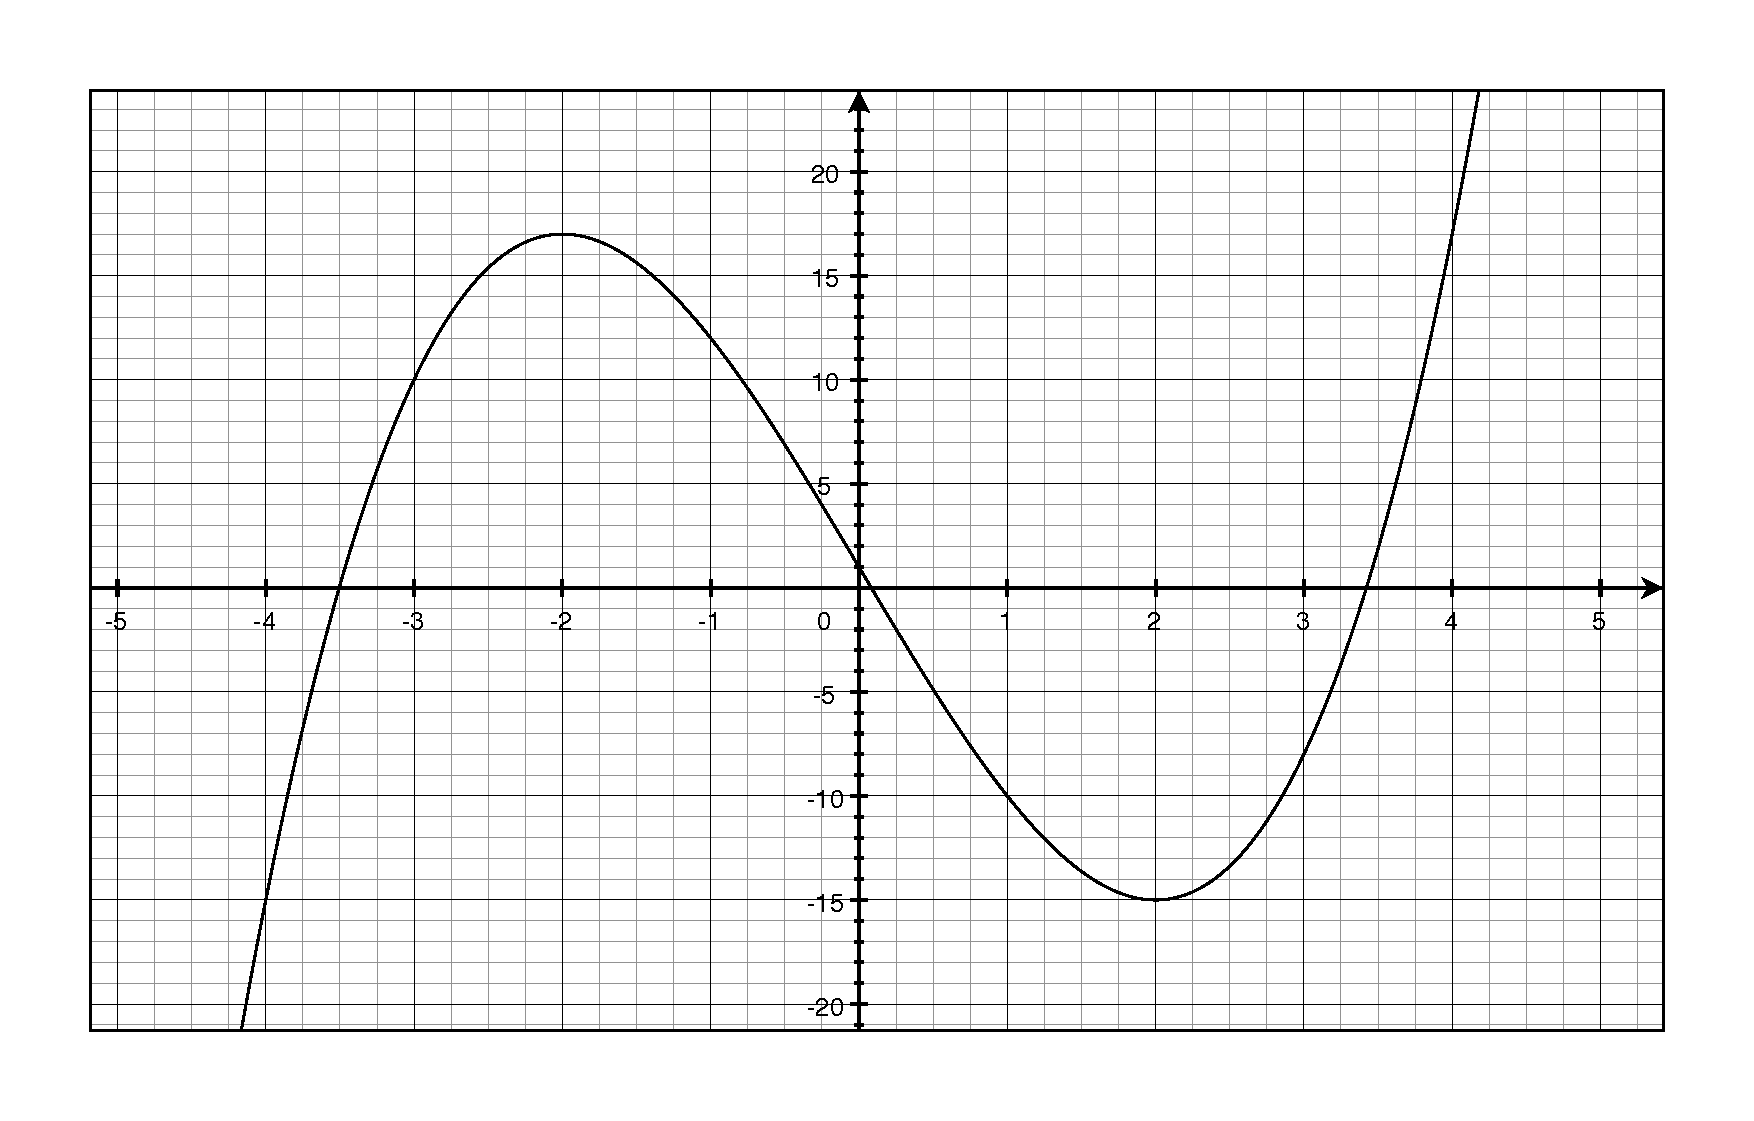
\includegraphics[scale=.3]{problem_19.eps}
  \caption*{Problem 19}
\end{figure}

\item[20]
\begin{align*}
  g(x)    &= 4x^3 - 3x^2 - 6x + 12 \\
  g'(x)   &= 12x^2 - 6x - 6 \\
  g''(x)  &= 24x - 6 \\
\end{align*}
\begin{align*}
  12x^2 - 6x - 6 &> 0 \\
  2x^2 - x - 1 &> 0 \\
  (2x + 1)(x - 1) &> 0 \\
  x < -\frac{1}{2} & \text{ or } x > 1 \\
\\
  24x - 6 &> 0 \\
  4x - 1 &> 0 \\
  x &> \frac{1}{4} \\
\end{align*}

\begin{tabular}{ll}
\toprule
increasing & $\left(-\infty, -\frac{1}{2} \right] \cup [1, \infty)$ \\
decreasing & $\left[ -\frac{1}{2}, 1 \right]$ \\
\midrule
concave up   & $\left(\frac{1}{4}, \infty \right)$ \\
concave down & $\left(-\infty, \frac{1}{4} \right)$ \\
\bottomrule
\end{tabular}

\begin{tabular}{lrrrrr}
\toprule
$x$    & -1 & -0.5  &  0 & 1 \\
$f(x)$ & 11 & 13.75 & 12 & 7 \\
\bottomrule
\end{tabular}

\begin{figure}[H]
  \centering
  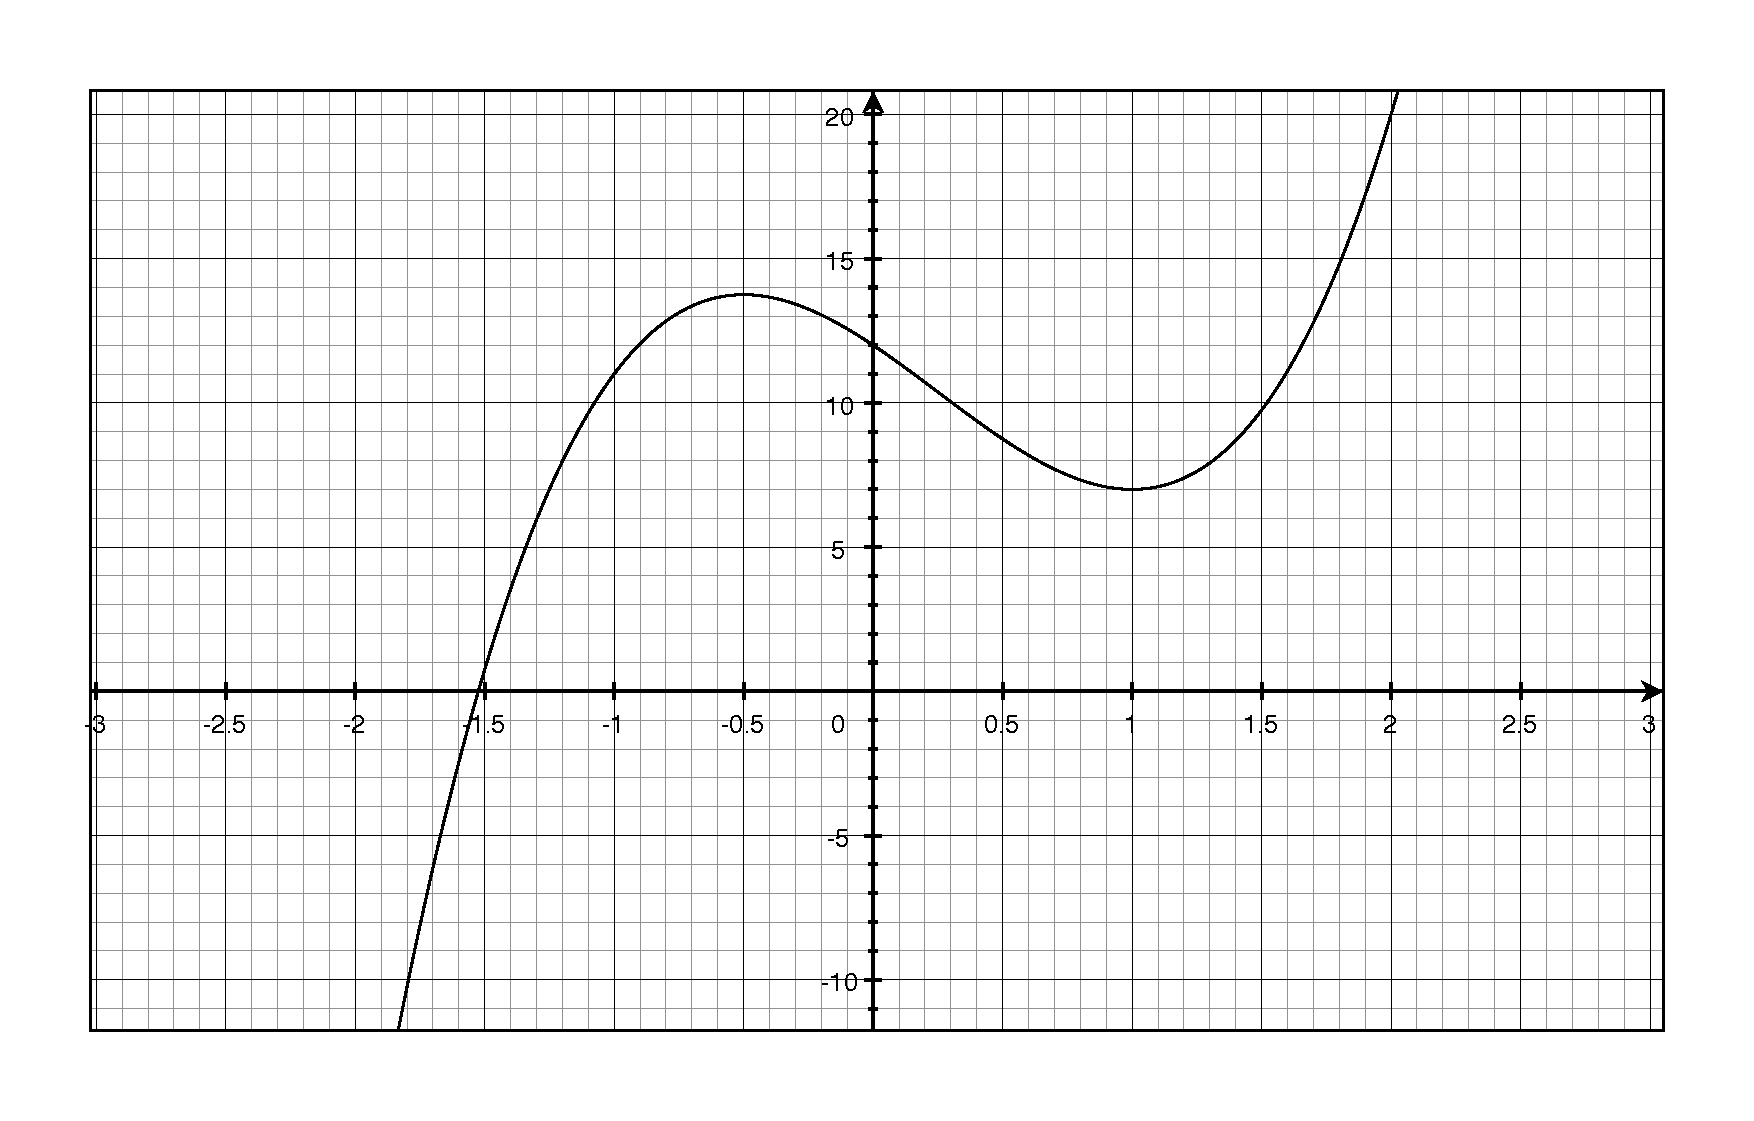
\includegraphics[scale=.3]{problem_20.eps}
  \caption*{Problem 20}
\end{figure}

\item[22]
\begin{align*}
  f(x)   &= x^6 - 3x^4    \\
  f'(x)  &= 6x^5 - 12x^3  \\
  f''(x) &= 30x^4 - 36x^2 \\
\end{align*}
\begin{align*}
  6x^5 - 12x^3 &> 0 \\
  x^5 - 2x^3 &> 0 \\
  x^3(x^2 - 2) &> 0 \\
  (2x + 1)(x - 1) &> 0 \\
  -\sqrt{2} < x < 0& \text{ or } x > \sqrt{2} \\
\\
  30x^4 - 36x^2 &> 0 \\
  5x^4 - 6x^2 &> 0 \\
  x^2(5x^2 - 6) &> 0 \\
  x^2 (\sqrt{5}x + \sqrt{6}) (\sqrt{5}x - \sqrt{6}) &> 0 \\
  x < -\sqrt{\frac{6}{5}} & \text{ or } x > \sqrt{\frac{6}{5}} \\
\end{align*}

\begin{tabular}{ll}
\toprule
increasing & $(-\sqrt{2}, 0) \cup (\sqrt{2}, \infty)$  \\
decreasing & $(-\infty, -\sqrt{2}) \cup (0, \sqrt{2})$ \\
\midrule
concave up   & $\left(- \infty, -\sqrt{\frac{6}{5}} \right) \cup \left( \sqrt{\frac{6}{5}}, \infty \right)$ \\
concave down & $\left(-\sqrt{\frac{6}{5}}, \sqrt{\frac{6}{5}} \right)$ \\
\bottomrule
\end{tabular}

This is an even function, so it is symmetric around the y-axis and we only need to evaluate points on one side of the
y-axis.

\begin{tabular}{lrrrrr}
\toprule
$x$    & 0 & 1  & $\sqrt{2}$ &  2 & \\
$f(x)$ & 0 & -2 &       $-4$ & 16 & \\
\bottomrule
\end{tabular}

\begin{figure}[H]
  \centering
  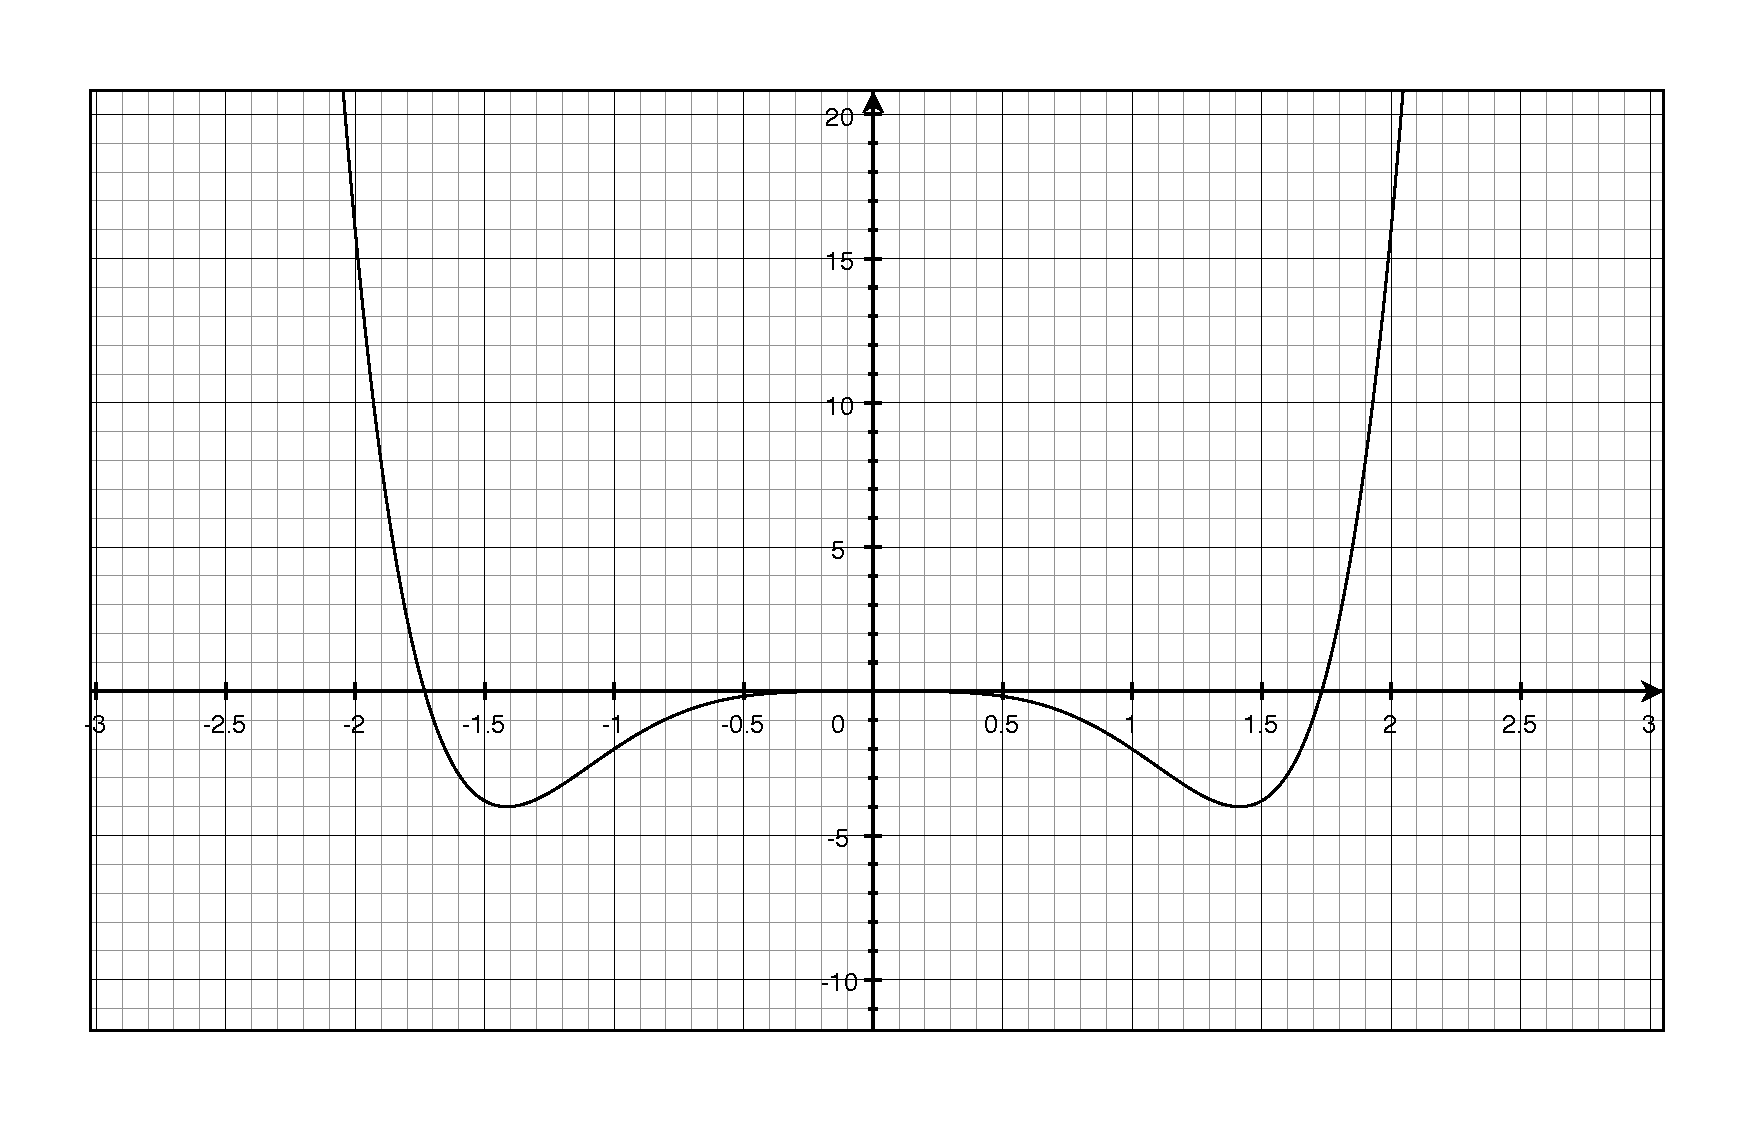
\includegraphics[scale=.3]{problem_22.eps}
  \caption*{Problem 22}
\end{figure}

\item[23]
\begin{align*}
  G(x)   &= 3x^5 - 5x^3 + 1 \\
  G'(x)  &= 15x^4 - 15x^2  \\
  G''(x) &= 60x^3 - 30x \\
\end{align*}
\begin{align*}
  15x^4 - 15x^2 &> 0 \\
  x^2(x^2 - 1) &> 0 \\
  x^2(x+1)(x - 1) &> 0 \\
  x < -1 & \text{ or } x > 1 \\
\\
  60x^3 - 30x &> 0 \\
  2x^3 - x &> 0 \\
  x(2x^2 - 1) &> 0 \\
  x(\sqrt{2} x + 1)(\sqrt{2} x - 1) &> 0 \\
  x^2 (\sqrt{5}x + \sqrt{6}) (\sqrt{5}x - \sqrt{6}) &> 0 \\
  -\frac{\sqrt{2}}{2} < x < 0 & \text{ or } x > \frac{\sqrt{2}}{2} \\
\end{align*}

$G'(0) = 0$, so $G$ is not increasing or decreasing at 0.

\begin{tabular}{ll}
\toprule
increasing & $(-\infty, -1] \cup [1, \infty)$  \\
decreasing & $[-1, 0) \cup (0, 1]$ \\
\midrule
concave up & $\left(-\frac{\sqrt{2}}{2}, 0 \right) \cup \left(\frac{\sqrt{2}}{2}, \infty \right)$ \\
concave down & $\left(-\infty, -\frac{\sqrt{2}}{2} \right) \cup \left(0, \frac{\sqrt{2}}{2} \right)$ \\
\bottomrule
\end{tabular}

\begin{tabular}{lrrrrr}
\toprule
$x$    & -1 & 0 &  1 \\
$f(x)$ &  3 & 1 & -1 \\
\bottomrule
\end{tabular}

\begin{figure}[H]
  \centering
  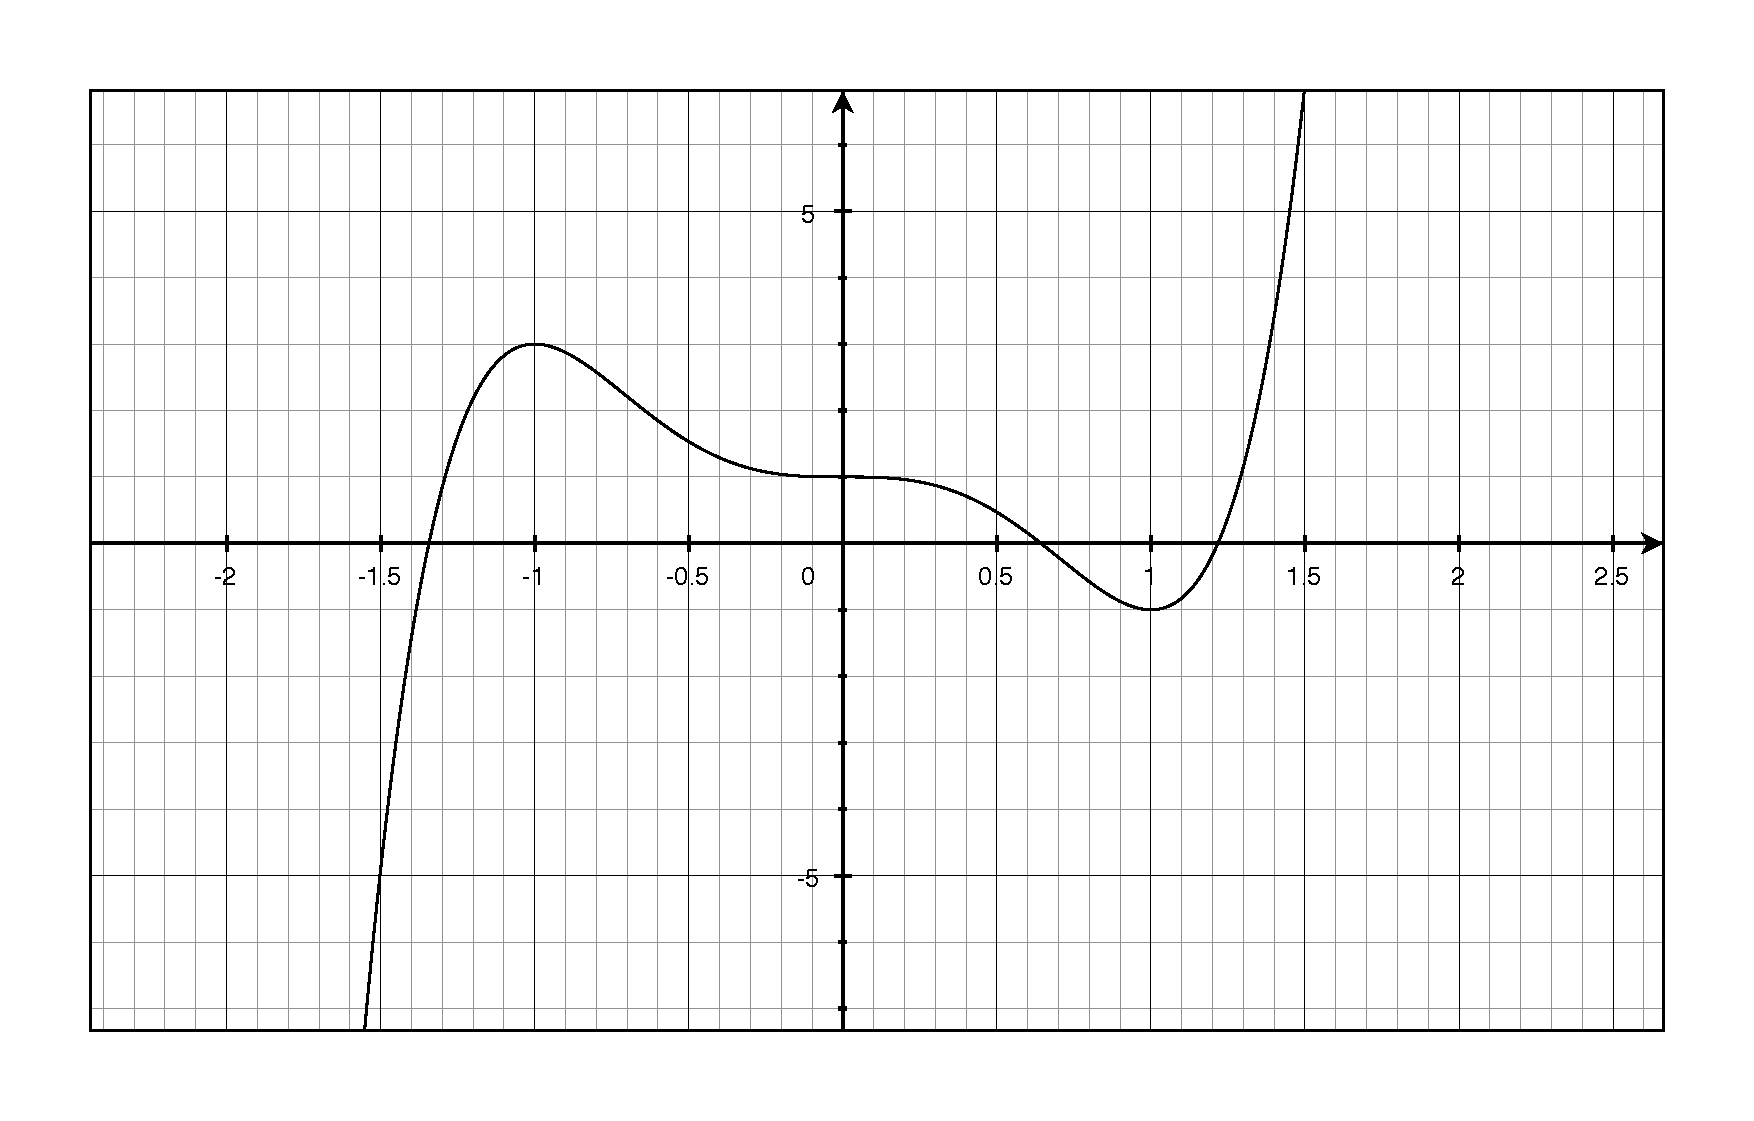
\includegraphics[scale=.3]{problem_23.eps}
  \caption*{Problem 23}
\end{figure}

\pagebreak

\item[25]
\begin{align*}
  f(x)   &= (\sin x)^{1/2} \\
  f'(x)  &= \frac{1}{2}(\sin x)^{-1/2}\cdot \cos x \\
         &= \frac{\cos x}{2 \sqrt{\sin x}} \\
  f''(x) &= -\frac{1}{2} \left( \sqrt{\sin x} + \frac{\cos^2 x}{\sqrt[3]{sin^2 x}} \right) \\
\end{align*}

\begin{itemize*}
  \item Since the denominator is always positive, $f'(x)$ has the same sign as its numerator.
  \item $f''(x)$ is always negative
\end{itemize*}

\begin{tabular}{ll}
\toprule
increasing & $\left[0, \frac{\pi}{2} \right]$ \\
decreasing & $\left[\frac{\pi}{2}, \pi \right]$ \\
\midrule
concave down & $(-\infty, \infty)$ \\
\bottomrule
\end{tabular}

\begin{tabular}{lrrrrr}
\toprule
$x$    & 0 & $\frac{\pi}{2}$ &  $\pi$ \\
$f(x)$ & 0 &               1 &     0  \\
\bottomrule
\end{tabular}

\begin{figure}[H]
  \centering
  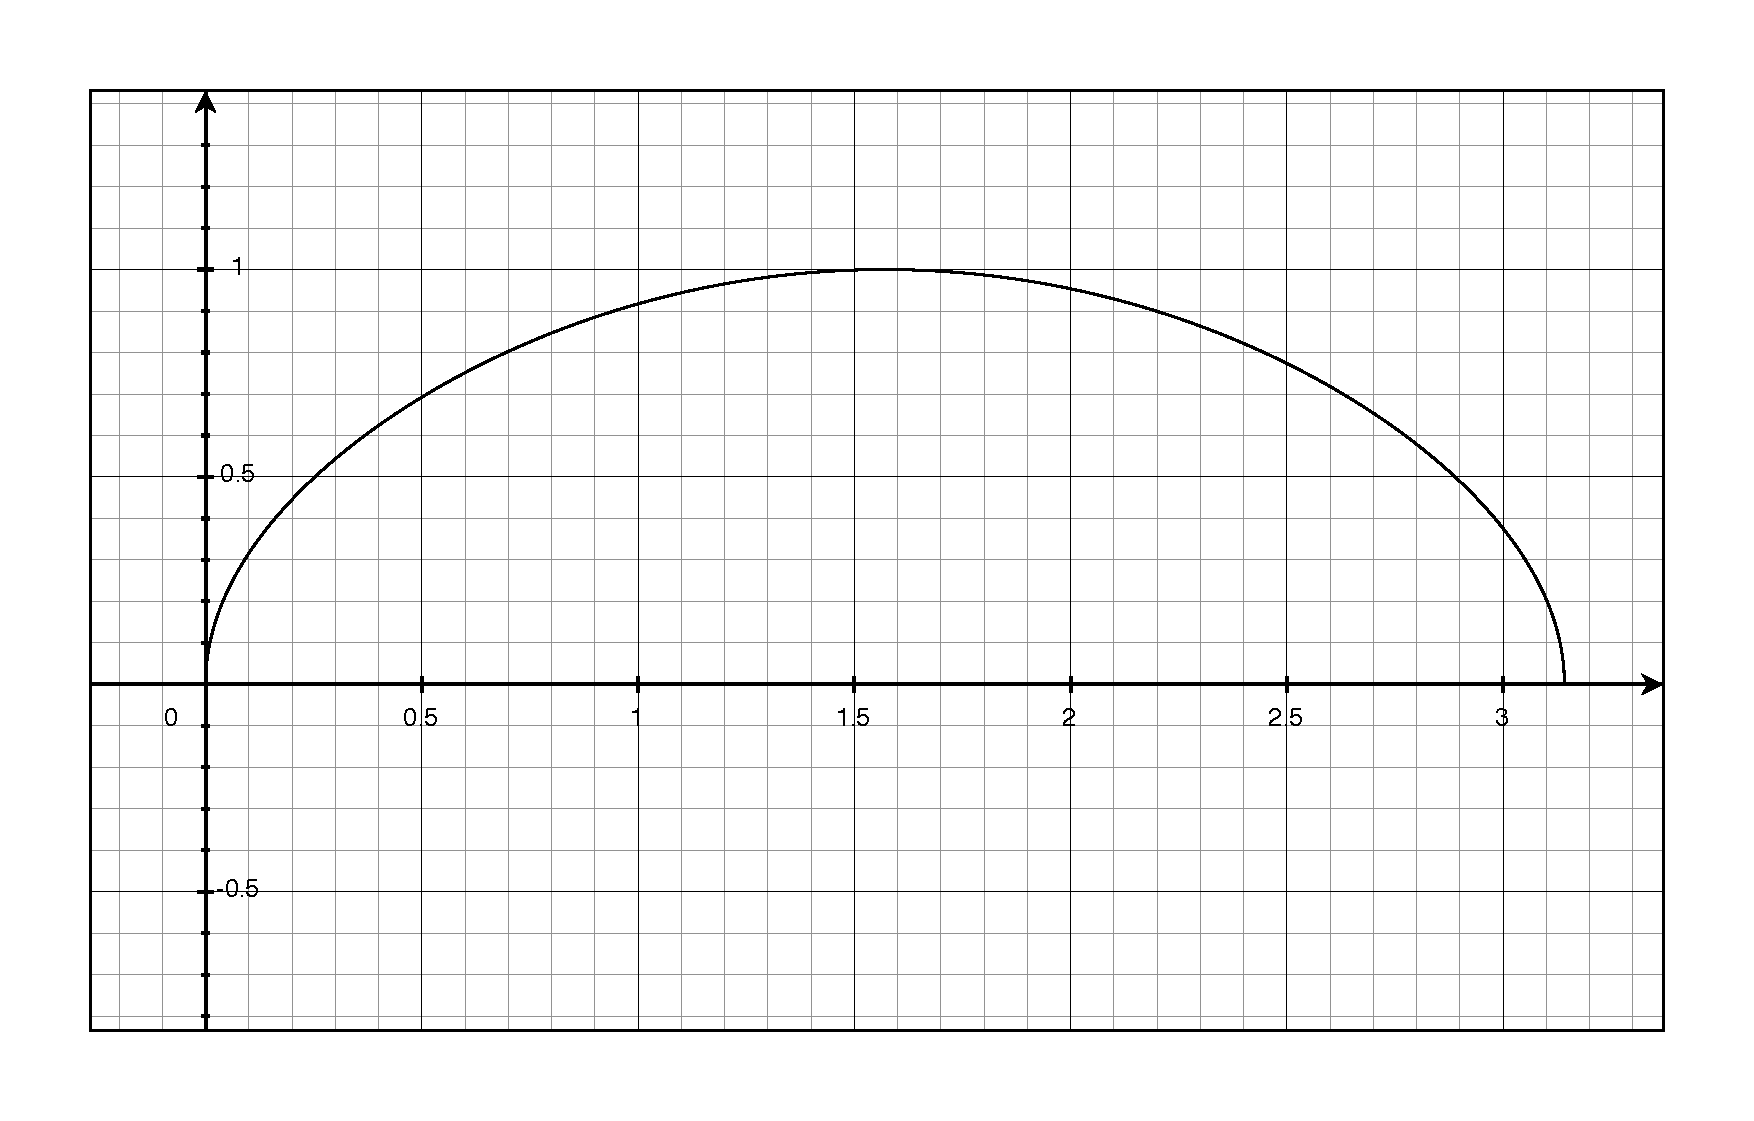
\includegraphics[scale=.3]{problem_25.eps}
  \caption*{Problem 25}
\end{figure}

\item[33]
\begin{align*}
  f(x)   &= ax^2 + bx + c \\
  f'(x)  &= 2ax + b \\
  f''(x) &= 2a \\
\end{align*}

$f''$ has whatever sign $a$ has for any value of $x$.  If $a < 0$, $f$ is always concave down and if $a > 0$, $f$ is always concave up.

\end{description}

\else

\vspace{4 cm}

{\em The word {\em anarchy} unsettles most people in the Western world;  it suggests disorder, violence, uncertainty.
  We have good reasons for fearing those conditions, because we have been living with them for a long time, not in
  anarchist societies (there have never been any) but in exactly those societies most fearful of anarchy---the powerful
  nation-states of modern times.}

\vspace{.2 cm}

\hspace{1 cm} --Howard Zinn

\fi

\end{document}

